\documentclass[a4paper]{article}
\usepackage{enumerate} %Let's us specify how to number enumerations
\usepackage{fullpage}  %Make the margins a bit smaller (not always sensible...)
\usepackage{graphicx}  %Ensures that \includegraphics will work
\usepackage{framed}
\usepackage{amsmath}
\usepackage{amsfonts}
\usepackage{bbm}
\usepackage{listings}
\usepackage{color}
\usepackage{amssymb}
\definecolor{dkgreen}{rgb}{0,0.6,0}
\definecolor{gray}{rgb}{0.5,0.5,0.5}
\definecolor{mauve}{rgb}{0.58,0,0.82}
\lstset{ %
  language=R,                     % the language of the code
  basicstyle=\footnotesize,       % the size of the fonts that are used for the code
  numbers=left,                   % where to put the line-numbers
  numberstyle=\tiny\color{gray},  % the style that is used for the line-numbers
  stepnumber=1,                   % the step between two line-numbers. If it's 1, each line
  numbersep=5pt,                  % how far the line-numbers are from the code
  backgroundcolor=\color{white},  % choose the background color. You must add \usepackage{color}
  showspaces=false,               % show spaces adding particular underscores
  showstringspaces=false,         % underline spaces within strings
  showtabs=false,                 % show tabs within strings adding particular underscores
  frame=single,                   % adds a frame around the code
  rulecolor=\color{black},        % if not set, the frame-color may be changed on line-breaks within not-black text (e.g. commens (green here))
  tabsize=2,                      % sets default tabsize to 2 spaces
  captionpos=b,                   % sets the caption-position to bottom
  breaklines=true,                % sets automatic line breaking
  breakatwhitespace=false,        % sets if automatic breaks should only happen at whitespace
  title=\lstname,                 % show the filename of files included with \lstinputlisting;
  keywordstyle=\color{blue},      % keyword style
  commentstyle=\color{dkgreen},   % comment style
  stringstyle=\color{mauve},      % string literal style
  escapeinside={\%*}{*)},         % if you want to add a comment within your code
  morekeywords={*,...}            % if you want to add more keywords to the set
} 

%You may also find the listings package useful for including sourcecode
 

\begin{document}
\title{Network Analytics}
\author{\bf Group 4}
\maketitle
\section*{Question 1}

\begin{enumerate}[(a)]
\item \textbf{Incidence Matrix}

We read the data into using the \texttt{read\_edgelist()} function and get the following incidence matrix.
\begin{table}[ht]
\begin{center}
\begin{tabular}{c|cccccccc}
a & 0 	& 0 	& 0 	& -1 	& 0\\
b &-1 	& -1	& 1 	& 1	&0\\
c &0 	& 1 	& 0 	& 0	&-1\\
d & 0 	& 0 	& -1 	& 0	& 1\\
e & 1 	& 0 	& 0 	& 0	& 0
\end{tabular}
\end{center}
\end{table}

\item \textbf{Shortest Path Matrix}

\begin{table}[ht]
\begin{center}
\begin{tabular}{c|cccccccc}
a & 0 	& $\inf$	& $\inf$	& $\inf$ & $\inf$\\
b &5 	& 0	& 6 	& 8	&$\inf$\\
c &15 	& 10 	& 0 	& 18	&$\inf$\\
d & 3 	& 8 	& -2 	& 0	&$ \inf$\\
e & 6 	& 7 	& 21	& 3	&$ \inf$
\end{tabular}
\end{center}
\end{table}

\item \textbf{Diameter}

Using the shortest path matrix above, we iterate through all values to find the maximum value while ignoring the $\infty$ values. The diameter of the graph is 18.

\item \textbf{Degree Distribution}

\begin{center}
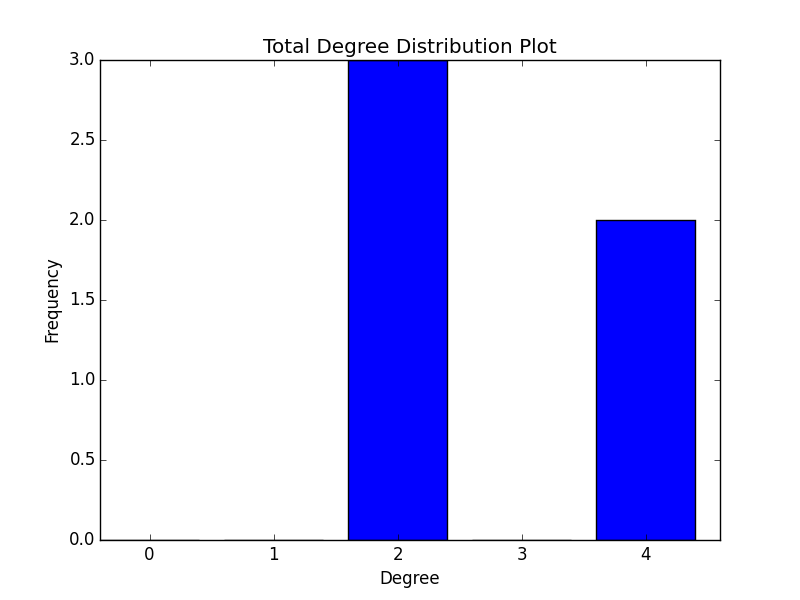
\includegraphics[width=100mm]{degree_histogram.png}
\end{center}

The support of the distribution is \{2,4\} with the probabilities,

$$\mathbb{P}(D=d)=
\begin{cases}
\frac{3}{5}, \text{if }d=2\\
\frac{2}{5}, \text{if }d=4
\end{cases}
$$

\item \textbf{Connectedness}

Using the commands \texttt{print(nx.is\_strongly\_connected(G))} and \texttt{print(nx.is\_weakly\_connected(G))}, we check both weak and strong connectivity. We find that the graph is WEAKLY connected but not STRONGLY connected due to the directed edges.

\end{enumerate}

\section*{Question 2}

\begin{center}
\includegraphics[width=100mm]{graph_plot.png}
\end{center}

All nodes in the graph are somewhat connected to each other. When using the shell layout, we find that the algorithm only generates one concentric circle, indicating the strong links between each node pairwise. Thus, the graph is best represented using this layout to display the  links between them.

\end{document}